\documentclass{article}
\usepackage[utf8x]{inputenc}
\usepackage{ucs}
\usepackage{amsmath} 
\usepackage{amsfonts}
\usepackage{marvosym}
\usepackage{wasysym}
\usepackage{upgreek}
\usepackage[english,russian]{babel}
\usepackage{graphicx}
\usepackage{float}
\usepackage{textcomp}
\usepackage{hyperref}
\usepackage{geometry}
  \geometry{left=2cm}
  \geometry{right=1.5cm}
  \geometry{top=1cm}
  \geometry{bottom=2cm}
\usepackage{tikz}
\usepackage{ccaption}
\usepackage{multicol}

\hypersetup{
   colorlinks=true,
   citecolor=blue,
   linkcolor=black,
   urlcolor=blue
}

\usepackage{listings}
%\setlength{\columnsep}{1.5cm}
%\setlength{\columnseprule}{0.2pt}

\usepackage[absolute]{textpos}

\usepackage{colortbl,graphicx,tikz}
\definecolor{X}{rgb}{.5,.5,.5}


\begin{document}
\pagenumbering{gobble}
\lstset{
  language=C,                % choose the language of the code
  basicstyle=\linespread{1.1}\ttfamily,
  columns=fixed,
  fontadjust=true,
  basewidth=0.5em,
  keywordstyle=\color{blue}\bfseries,
  commentstyle=\color{gray},
  stringstyle=\ttfamily\color{orange!50!black},
  showstringspaces=false,
  numbersep=5pt,
  numberstyle=\tiny\color{black},
  numberfirstline=true,
  stepnumber=1,                   % the step between two line-numbers.        
  numbersep=10pt,                  % how far the line-numbers are from the code
  backgroundcolor=\color{white},  % choose the background color. You must add \usepackage{color}
  showstringspaces=false,         % underline spaces within strings
  captionpos=b,                   % sets the caption-position to bottom
  breaklines=true,                % sets automatic line breaking
  breakatwhitespace=true,         % sets if automatic breaks should only happen at whitespace
  xleftmargin=.2in,
  extendedchars=\true,
  keepspaces = true,
}
\lstset{literate=%
   *{0}{{{\color{red!20!violet}0}}}1
    {1}{{{\color{red!20!violet}1}}}1
    {2}{{{\color{red!20!violet}2}}}1
    {3}{{{\color{red!20!violet}3}}}1
    {4}{{{\color{red!20!violet}4}}}1
    {5}{{{\color{red!20!violet}5}}}1
    {6}{{{\color{red!20!violet}6}}}1
    {7}{{{\color{red!20!violet}7}}}1
    {8}{{{\color{red!20!violet}8}}}1
    {9}{{{\color{red!20!violet}9}}}1
}
\newpage

\title{Семинар \#9: Бинарные файлы и изображения. Классные задания.\vspace{-5ex}}\date{}\maketitle

\section*{Часть 1: Переменные в памяти. Little и Big Endian}
Положение любой переменной в памяти характеризуется двумя числами: её адресом(номером первого байта этой переменной) и её размером. Рассмотрим ситуацию, когда были созданы 3 переменные типов \texttt{int} (размер 4 байта), \texttt{char} (размер 1 байт) и \texttt{float} (размер 4 байта).
На рисунке представлено схематическое расположение этих переменных в памяти (одному квадратику соответствует 1 байт):

\begin{center}
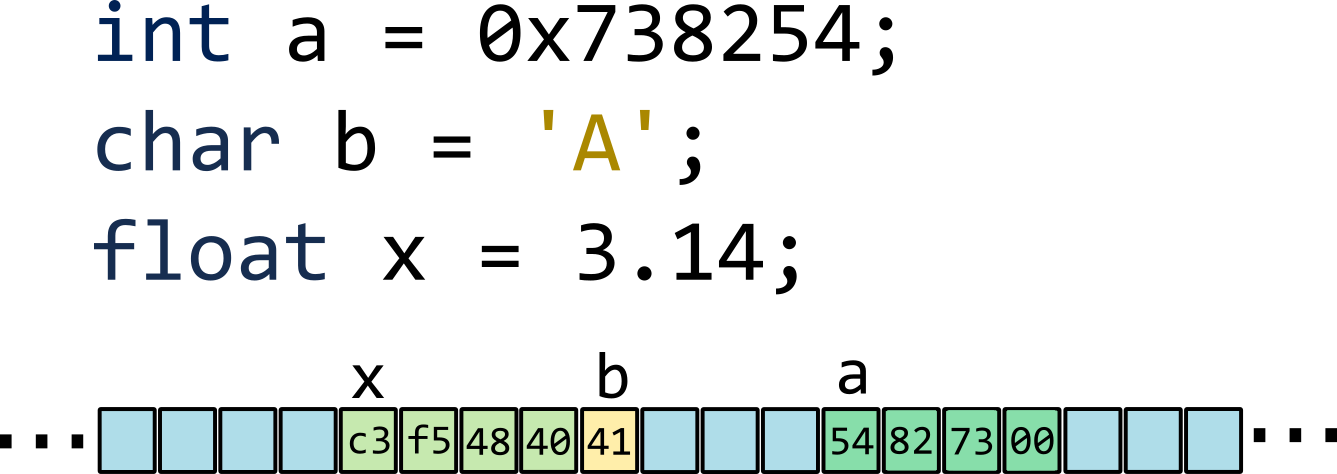
\includegraphics[scale=1]{../images/memory/memory_2_different_types.png}
\end{center}
Какие выводы можно сделать из этого изображения:
\begin{itemize}
\item Значение одного байта памяти удобно представлять двузначным шестнадцатиричным числом.
\item Каждая переменная заняла столько байт, чему равен её размер.
\item Переменные в памяти могут хранится не в том порядке, в котором вы их объявляете.
\item Переменные в памяти хранятся не обязательно вплотную друг к другу.
\item Байты переменных \texttt{a} и \texttt{b} хранятся в обратном порядке. Такой порядок байт называется \texttt{Little Endian}.  Обратите внимание, что обращается только порядок байт, а не бит. Большинство компьютеров применяют именно такой порядок байт. Но в некоторых системах может использоваться обычный порядок байт -- \texttt{Big Endian}. Обратный порядок байт применяется не только к типу \texttt{int}, но и ко всем базовым типам.
\item Переменная \texttt{b} хранит ASCII-код символа \texttt{A}. Он который равен $65 = 41_{16}$.
\end{itemize}


\newpage
\section*{Часть 2: Просмотр байт}
\subsection*{Просмотр байт переменной}
Просмотреть, что содержится в байтах какого-либо объекта можно с помощью указателя на \texttt{unsigned char}.

\begin{lstlisting} 
#include <stdio.h>
int main() 
{
    int a = 0x11223344;
    
    unsigned char* p = (unsigned char*)&a;
    for (size_t i = 0; i < sizeof(a); ++i)
        printf("%x ", *(p + i));
    printf("\n");
}
\end{lstlisting}

\subsubsection*{Задача:}

\begin{itemize}
\item Напечатайте байты объекта \texttt{a} типа \texttt{double}.
\begin{lstlisting} 
double a = 123.456;
\end{lstlisting}

\item Напечатайте байты объекта \texttt{b} типа \texttt{int}.
\begin{lstlisting} 
int b = -1;
\end{lstlisting}

\item Напечатайте байты объекта \texttt{c} типа \texttt{struct cat}.
\begin{lstlisting} 
struct cat
{
    char first;
    int second;
};

int main()
{
    struct cat c = {0x50, 0x12345678}
}

\end{lstlisting}


\end{itemize}



\section*{Часть 3: Работа с памятью. Стандартные функции \texttt{memset}, \texttt{memcpy} и \texttt{memmove}.}




\newpage
\section*{Часть 4: Работы с бинарными файлами \texttt{fread} и \texttt{fwrite}}
\texttt{fwrite} записывает некоторый участок памяти в файл без обработки. \\
\texttt{fread} считывает данные из файла в память без обработки.

Пример. Записываем 4 байта памяти переменной \texttt{a} в файл \texttt{binary.dat}:
\begin{lstlisting}
#include <stdio.h>
int main() 
{
    int a = 0x11223344;
    FILE* fb = fopen("binary.dat", "wb");
    fwrite(&a, sizeof(int), 1, fb);
    fclose(fb);
}
\end{lstlisting}

\begin{itemize}
\item \textbf{Печать в текстовом и бинарном виде:}\\
В файле \texttt{text\_and\_binary.c} содержится пример записи числа в текстовом и бинарном виде. Скомпилируйте эту программу и запустите. Должно появиться 2 файла (\texttt{number.txt} и \texttt{number.bin}). Изучите оба эти файла, открывая их в текстовом редакторе, а также с помощью утилиты \texttt{xxd}. Объясните результат.


\item \textbf{Печать массива в бинарном виде:}\\
Пусть есть массив из чисел типа \texttt{int}: \texttt{int array[5] = \{111, 222, 333, 444, 555\};}\\
Запишите эти числа в текстовый файл \texttt{array.txt}, используя \texttt{fprintf}. Изучите содержимое этого файла побайтово с помощью \texttt{xxd}.\\
Запишите эти числа в бинарный файл \texttt{array.bin}, используя \texttt{fwrite}. Изучите содержимое этого файла побайтово с помощью \texttt{xxd}.
\end{itemize}






\newpage
\section*{Часть 3: Работа с изображениями формата \texttt{.ppm}}
Простейший формат для изображение имеет следующую структуру
\begin{verbatim}
P3
3 2
255
255 0 0 
0 255 0  
0 0 255 
255 255 0 
255 255 255 
0 0 0
\end{verbatim}
\begin{itemize}
\item В первой строке задаётся тип файла \texttt{P3} - означает, что в этом файле будет храниться цветное изображение, причём значения пикселей будет задаваться в текстовом формате.
\item Во второй строке задаются размеры картинки - 3 на 2 пикселя.
\item Во третьей строке задаётся максимальное значение RGB компоненты цвета.
\item Дальше идут RGB компоненты цветов каждого пикселя в текстовом формате.
\end{itemize}
Картинка имеет следующий вид:
\begin{center}

\includegraphics[scale=0.5]{../images/tiny.png}
\end{center}

\subsection*{Задачи}
\begin{itemize}
\item Написать программу, которая генерирует одноцветную картинку (500 на 500) в формате \texttt{.ppm}. Цвет должен передаваться через аргументы командной строки.
\item \textbf{Белый шум:} Написать программу, которая случайное изображение в формате \texttt{.ppm}. Цвет каждого пикселя задаётся случайно.
\item \textbf{Градиент:} Написать программу, которая генерирует градиентную картинку в формате \texttt{.ppm}. Два цвета должны передаваться через аргументы командной строки.
\item \textbf{Черно-белая картинка:} Написать программу, которая считывает изображение в формате \texttt{.ppm} и сохраняет его в черно-белом виде. Файл изображения должен передаваться через аргументы командной строки. Считайте файл \texttt{russian\_peasants\_1909.ppm} и сделайте его черно-белым.
\end{itemize}


\newpage
\section*{Часть 4: Работа с изображениями формата \texttt{.jpeg}}




\end{document}